\mode<article>{
\clearpage
}

\section{Temporal decoupling and the quantum keeper}

\mode<presentation>{

\begin{frame}
	\frametitle{Temporal decoupling and Quantum Keeper}
	\begin{block}{Temporal decoupling}
		Technique to enhance simulation speed specially adapted for the loosely-timed coding style.\newline
		It allows TLM models to run ahead of the current simulation time without yielding control to the simulation engine (i.e., without calling \texttt{wait(\ldots)}.
	\end{block}
\end{frame}

\begin{frame}
	\frametitle{Temporal decoupling example}
	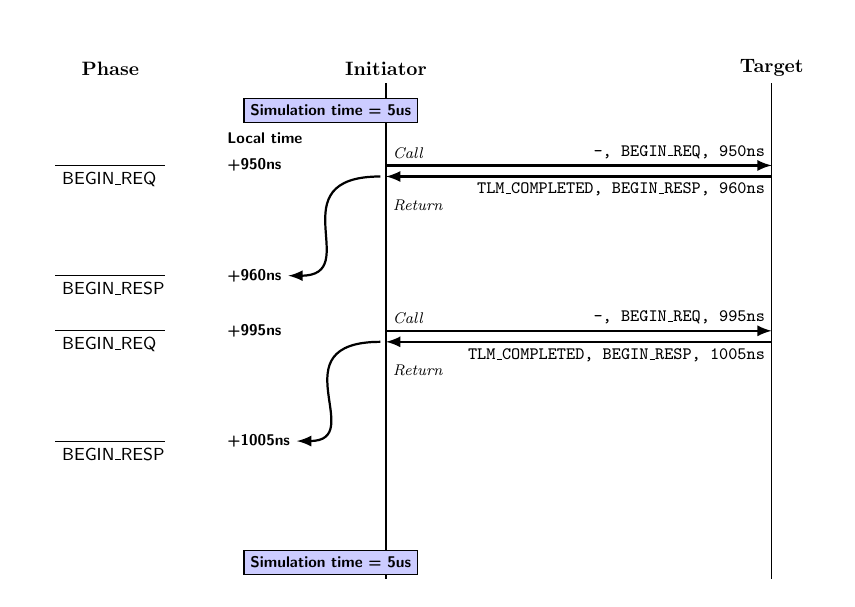
\begin{tikzpicture}[transform shape, scale=0.7]
		\clip (0.5,0) rectangle (15,10);
%		\draw[help lines] (0,0) grid (15,10);
		\path (2,9) coordinate (phase);
		\path (1,7.5) coordinate (req0);
		\path (3,7.5) coordinate (req1);
		\path (1,5.5) coordinate (rsp0);
		\path (3,5.5) coordinate (rsp1);
		\path (1,4.5) coordinate (req1_0);
		\path (3,4.5) coordinate (req1_1);
		\path (1,2.5) coordinate (rsp1_0);
		\path (3,2.5) coordinate (rsp1_1);
		\path (4,8) node(local_time) [right] {\footnotesize \textsf{\textbf{Local time}}};
		\path (4,7.5) node(10ns) [right] {\footnotesize \textsf{\textbf{+950ns}}};
		\path (4,5.5) node(20ns) [right] {\footnotesize \textsf{\textbf{+960ns}}};
		\path (4,4.5) node(35ns) [right] {\footnotesize \textsf{\textbf{+995ns}}};
		\path (4,2.5) node(45ns) [right] {\footnotesize \textsf{\textbf{+1005ns}}};
%		\path (4,1) node(wait) [right] {\footnotesize \textsf{\textbf{wait(1us)}}};
		\path (7,0) coordinate (llb);
		\path (7,9) coordinate (llt);
		\path (14,0) coordinate (rlb);
		\path (14,9) coordinate (rlt);
		\path (7,7.5) coordinate (call_left);
		\path (14,7.5) coordinate (call_right);
		\path (7,7.3) coordinate (ret_left);
		\path (14,7.3) coordinate (ret_right);
		\path (7,4.5) coordinate (call2_left);
		\path (14,4.5) coordinate (call2_right);
		\path (7,4.3) coordinate (ret2_left);
		\path (14,4.3) coordinate (ret2_right);

		\draw (phase) node[above] {\textbf{Phase}};
		\draw (llb) -- (llt)
			node[above] {\textbf{Initiator}};
		\draw (rlb) -- (rlt)
			node[above] {\textbf{Target}};
		\draw (req0) node[below right] {\small \textsf{BEGIN\_REQ}} -- (req1);
		\draw (rsp0) node[below right] {\small \textsf{BEGIN\_RESP}} -- (rsp1);
		\draw (req1_0) node[below right] {\small \textsf{BEGIN\_REQ}} -- (req1_1);
		\draw (rsp1_0) node[below right] {\small \textsf{BEGIN\_RESP}} -- (rsp1_1);
		\draw[thick,-latex] (call_left) -- (call_right);
		\draw (call_left) node[above right] {\footnotesize \emph{Call}};
		\draw (call_right) node[above left] {\small \texttt{\textbf{-, BEGIN\_REQ, 950ns}}};
		\draw[thick,latex-] (ret_left) -- (ret_right);
		\draw (ret_left) +(0,-0.3) node[below right] {\footnotesize \emph{Return}};
		\draw (ret_right) node[below left] {\small \texttt{\textbf{TLM\_COMPLETED, BEGIN\_RESP, 960ns}}};
		\draw[thick,-latex] (call2_left) -- (call2_right);
		\draw (call2_left) node[above right] {\footnotesize \emph{Call}};
		\draw (call2_right) node[above left] {\small \texttt{\textbf{-, BEGIN\_REQ, 995ns}}};
		\draw[thick,latex-] (ret2_left) -- (ret2_right);
		\draw (ret2_left) +(0,-0.3) node[below right] {\footnotesize \emph{Return}};
		\draw (ret2_right) node[below left] {\small \texttt{\textbf{TLM\_COMPLETED, BEGIN\_RESP, 1005ns}}};
		\path (6,8.5) node(100ns) [rectangle,draw,fill=blue!20] {\footnotesize \textsf{\textbf{Simulation time = 5us}}};
		\path (6,0.3) node(110ns) [rectangle,draw,fill=blue!20] {\footnotesize \textsf{\textbf{Simulation time = 5us}}};
		\path (ret_left) +(-2,0) coordinate (control_ret_left);
		\path (20ns) +(2,0) coordinate (control_20ns);
		\draw[thick,-latex] (ret_left) +(-0.1,0) .. controls (control_ret_left) and (control_20ns) .. (20ns)[above];
		\path (ret2_left) +(-2,0) coordinate (control_ret2_left);
		\path (45ns) +(2,0) coordinate (control_45ns);
		\draw[thick,-latex] (ret2_left) +(-0.1,0) .. controls (control_ret2_left) and (control_45ns) .. (45ns)[above];
	\end{tikzpicture}
\end{frame}

\begin{frame}
	\frametitle{Temporal decoupling and Quantum Keeper}
	\begin{block}{Temporal decoupling}
		Technique to enhance simulation speed specially adapted for the loosely-timed coding style.\newline
		It allows TLM models to run ahead of the current simulation time without yielding control to the simulation engine (i.e., without calling \texttt{wait(\ldots)}.
	\end{block}
	\alert{Beware of process inanition.}
	\begin{itemize}
		\item<2-> Solution:
		\begin{itemize}
			\item<2-> The Quantum Keeper
		\end{itemize}
	\end{itemize}
\end{frame}

\begin{frame}
	\frametitle{The Quantum Keeper (\texttt{tlm\_quantum\_keeper})}
	\begin{itemize}
		\item Convenience class to control avoid inanition.
	\end{itemize}
	\lstinputlisting{tlm/quantum_keeper.hh}
\end{frame}

\begin{frame}
	\frametitle{Quantum Keeper example}
	\lstinputlisting[linerange={1-14, 36-37}]{tlm/quantum_keeper_example.hh}
\end{frame}

\begin{frame}
	\frametitle{Quantum Keeper example (cont.)}
	\lstinputlisting[linerange={1-3, 15-37}]{tlm/quantum_keeper_example.hh}
\end{frame}
}

\mode<article>{
\emph{Temporal decoupling} is a powerful technique to enhance SystemC simulation speed specially adapted for the loosely-timed coding style.
Basically it consist on doing as much work as possible inside a module process without yielding the control to the SystemC simulation engine\footnote{That is, without performing any call to \texttt{wait(\ldots)}.}.
So this technique allows TLM models to run ahead of the current simulation time (as it is returned by \texttt{sc\_time\_stamp()}).

\begin{figure}[h]
	\begin{center}
	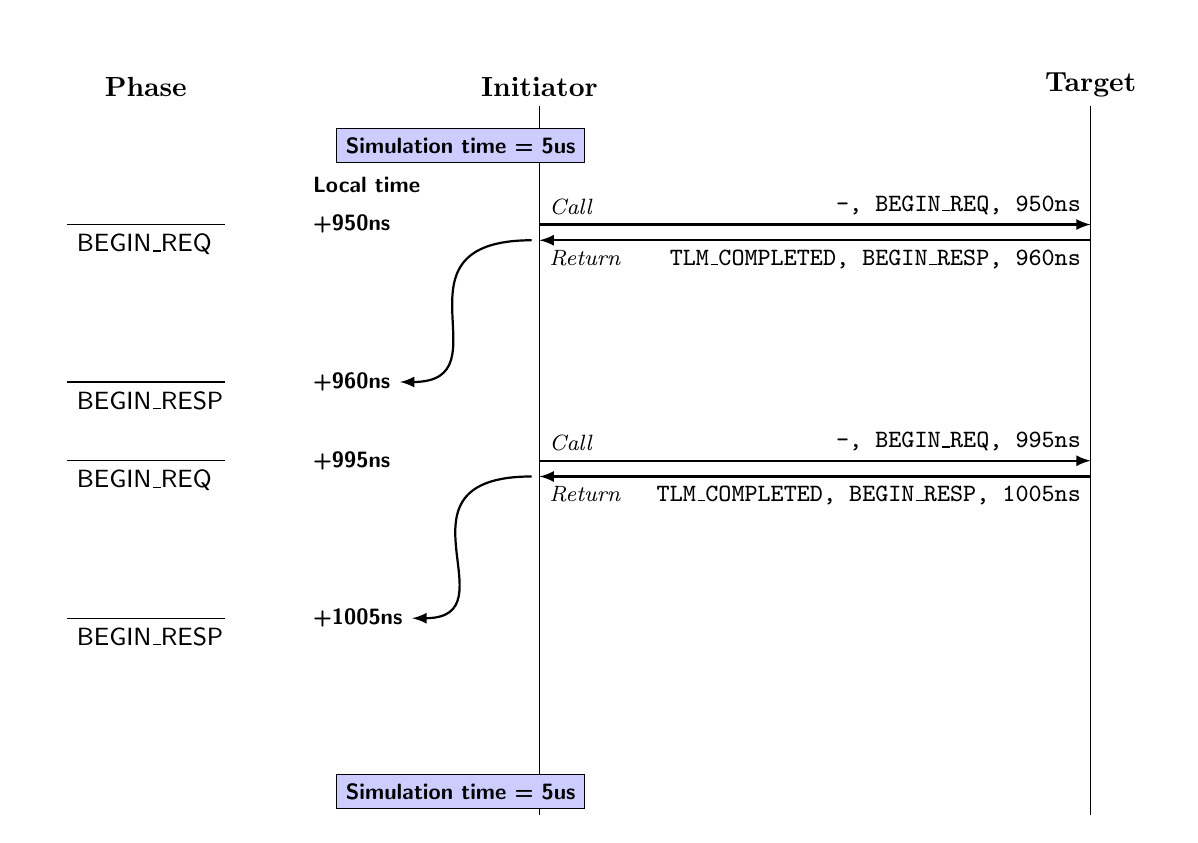
\begin{tikzpicture}
		\clip (0.5,0) rectangle (15,10);
%		\draw[help lines] (0,0) grid (15,10);
		\path (2,9) coordinate (phase);
		\path (1,7.5) coordinate (req0);
		\path (3,7.5) coordinate (req1);
		\path (1,5.5) coordinate (rsp0);
		\path (3,5.5) coordinate (rsp1);
		\path (1,4.5) coordinate (req1_0);
		\path (3,4.5) coordinate (req1_1);
		\path (1,2.5) coordinate (rsp1_0);
		\path (3,2.5) coordinate (rsp1_1);
		\path (4,8) node(local_time) [right] {\footnotesize \textsf{\textbf{Local time}}};
		\path (4,7.5) node(10ns) [right] {\footnotesize \textsf{\textbf{+950ns}}};
		\path (4,5.5) node(20ns) [right] {\footnotesize \textsf{\textbf{+960ns}}};
		\path (4,4.5) node(35ns) [right] {\footnotesize \textsf{\textbf{+995ns}}};
		\path (4,2.5) node(45ns) [right] {\footnotesize \textsf{\textbf{+1005ns}}};
%		\path (4,1) node(wait) [right] {\footnotesize \textsf{\textbf{wait(1us)}}};
		\path (7,0) coordinate (llb);
		\path (7,9) coordinate (llt);
		\path (14,0) coordinate (rlb);
		\path (14,9) coordinate (rlt);
		\path (7,7.5) coordinate (call_left);
		\path (14,7.5) coordinate (call_right);
		\path (7,7.3) coordinate (ret_left);
		\path (14,7.3) coordinate (ret_right);
		\path (7,4.5) coordinate (call2_left);
		\path (14,4.5) coordinate (call2_right);
		\path (7,4.3) coordinate (ret2_left);
		\path (14,4.3) coordinate (ret2_right);

		\draw (phase) node[above] {\textbf{Phase}};
		\draw (llb) -- (llt)
			node[above] {\textbf{Initiator}};
		\draw (rlb) -- (rlt)
			node[above] {\textbf{Target}};
		\draw (req0) node[below right] {\small \textsf{BEGIN\_REQ}} -- (req1);
		\draw (rsp0) node[below right] {\small \textsf{BEGIN\_RESP}} -- (rsp1);
		\draw (req1_0) node[below right] {\small \textsf{BEGIN\_REQ}} -- (req1_1);
		\draw (rsp1_0) node[below right] {\small \textsf{BEGIN\_RESP}} -- (rsp1_1);
		\draw[thick,-latex] (call_left) -- (call_right);
		\draw (call_left) node[above right] {\footnotesize \emph{Call}};
		\draw (call_right) node[above left] {\small \texttt{\textbf{-, BEGIN\_REQ, 950ns}}};
		\draw[thick,latex-] (ret_left) -- (ret_right);
		\draw (ret_left) node[below right] {\footnotesize \emph{Return}};
		\draw (ret_right) node[below left] {\small \texttt{\textbf{TLM\_COMPLETED, BEGIN\_RESP, 960ns}}};
		\draw[thick,-latex] (call2_left) -- (call2_right);
		\draw (call2_left) node[above right] {\footnotesize \emph{Call}};
		\draw (call2_right) node[above left] {\small \texttt{\textbf{-, BEGIN\_REQ, 995ns}}};
		\draw[thick,latex-] (ret2_left) -- (ret2_right);
		\draw (ret2_left) node[below right] {\footnotesize \emph{Return}};
		\draw (ret2_right) node[below left] {\small \texttt{\textbf{TLM\_COMPLETED, BEGIN\_RESP, 1005ns}}};
		\path (6,8.5) node(100ns) [rectangle,draw,fill=blue!20] {\footnotesize \textsf{\textbf{Simulation time = 5us}}};
		\path (6,0.3) node(110ns) [rectangle,draw,fill=blue!20] {\footnotesize \textsf{\textbf{Simulation time = 5us}}};
		\path (ret_left) +(-2,0) coordinate (control_ret_left);
		\path (20ns) +(2,0) coordinate (control_20ns);
		\draw[thick,-latex] (ret_left) +(-0.1,0) .. controls (control_ret_left) and (control_20ns) .. (20ns)[above];
		\path (ret2_left) +(-2,0) coordinate (control_ret2_left);
		\path (45ns) +(2,0) coordinate (control_45ns);
		\draw[thick,-latex] (ret2_left) +(-0.1,0) .. controls (control_ret2_left) and (control_45ns) .. (45ns)[above];
	\end{tikzpicture}
	\end{center}
	\caption{Loosely-timed coding style with temporal decoupling example.}
	\label{fig:temporal_decoupling_example}
\end{figure}

Figure~\ref{fig:temporal_decoupling_example} shows an example of a loosely-timed coding style model using temporal decoupling.
However, this technique can be dangerous, producing inanition of other processes which are waiting for SystemC to execute them.
Simply imagine that the initiator in Figure~\ref{fig:temporal_decoupling_example} never performs a \texttt{wait(\ldots)} and other initiator processes in the system never get execution.
So, when using the temporal decoupling technique care must be taken to avoid inanition.

\begin{figure}[h]
	\lstinputlisting{tlm/quantum_keeper.hh}
	\caption{The quantum keeper class definition.}
	\label{fig:quantum_keeper_definition}
\end{figure}

To facilitate the task of avoiding inanition, TLM 2.0 provides the convenience class \texttt{tlm\_quantum\_keeper} (aka. The Quantum Keeper).
It provides a set of methods for managing and interacting with the time quantum. 
It is recommended to use it in order to maintain a consistent coding style (but not compulsory).
Figure~\ref{fig:quantum_keeper_definition} shows the class definition of the quantum keeper.

\begin{figure}[h]
	\lstinputlisting{tlm/quantum_keeper_example.hh}
	\caption{Example of a loosely-timed initiator using the quantum keeper.}
	\label{fig:quantum_keeper_example}
\end{figure}

Basically this class keeps track of the module local time and synchronizes when necessary with the SystemC simulation time when necessary.
The user must define the time threshold the modules can run ahead of time using the static method \texttt{set\_global\_quantum}.
When the module local time difference with the simulation time reaches the user defined threshold the quantum keeper notifies the module that it must synchronize, that is, that is must perform a \texttt{wait(\ldots)} with the amount of time signaled by the quantum keeper.
Figure~\ref{fig:quantum_keeper_example} shows the example of a loosely-timed initiator using the quantum keeper.

Note that the user must define the time threshold for the quantum keeper globally, so no module should ever call the \texttt{set\_global\_quantum}.
Usually the quantum keeper time threshold is set up globally before or after the assembly of the simulator modules and before calling \texttt{sc\_start}.
To have a global quantum keeper time threshold helps to avoid inanition, because all the modules will share the same threshold.
The threshold is also a toggle between simulation speed and simulation accuracy, the bigger its value the less modules will yield and the faster the simulation will be. 
The smaller its value the more modules will yield and the slower the simulation will be.
}
